\documentclass[3p, twocolumn]{elsarticle}
\usepackage{ae,aecompl}
\usepackage[T1]{fontenc}
\usepackage[utf8]{inputenc}
\usepackage{pgfplots}
\usepackage{pst-plot}
\usepackage{tikz}
\usepgfplotslibrary{external}
\tikzexternalize
\usepackage{amsmath}
\usepackage{amssymb}
\usepackage{gensymb}
\usepackage{upgreek}
\usepackage{float}
\usepackage{indentfirst}
\parskip=0pt
\usepackage[colorlinks = true,
            linkcolor = red,
            urlcolor  = blue,
            citecolor = blue,
            anchorcolor = blue]{hyperref}

\begin{document}

\begin{frontmatter}

\title{Potentiometric Scanning Electrochemical Microscopic Mapping of the Distributed Belousov-Zhabotinsky Oscillating Reaction}
\cortext[cor]{Corresponding author}
\author[akiss]{András Kiss\corref{cor}}
\ead{akiss@gamma.ttk.pte.hu}
\author[szszilard]{Szilárd Szili}
\address[akiss, gnagy, szszilard]{Department of General and Physical Chemistry, Faculty of Sciences, University of Pécs, 7624 Pécs, Ifjúság útja 6, Hungary}
\address[akiss, gnagy]{János Szentágothai Research Centre, University of Pécs, 7624 Pécs, Ifjúság Útja 20, Hungary}
\author[gnagy]{Géza Nagy}
\ead{g-nagy@gamma.ttk.pte.hu}

\begin{abstract}

Patterns emerging in a distributed Belousov-Zhabotinsky reaction are usually studied with optical methods.
However, these methods provide only approximate information about the oxidation state of an indicator, and they cannot be applied when there is no indicator dye or other colored component whose concentration is oscillating.
To gather additional information about the processes involved in the reaction, electrochemical methods have been used by many research groups.
%Using the appropriate electrodes, changes in bromide ion activity, pH and redox potential can be monitored.
Unfortunately, these methods will influence a distributed system, since they require electrodes to be placed inside the reaction mixture.
The electrodes -- depending on their size -- will influence the formation of spatial patterns, especially if one of them moves, for instance when used as a measuring tip in scanning electrochemical microscopy (SECM).
%This poses no problem when the studied reaction is stirred, but in a distributed system the electrodes -- depending on their size -- will influence the formation of spatial patterns, especially if one of them moves, for instance when used as a measuring tip in scanning electrochemical microscopy (SECM).

The aim of this paper is to show that the advantages of optical and electrochemical methods can be combined.
That is, spatially resolved electrochemical data can be gathered of certain species in the reaction.
Furthermore, in this paper we show that, using a sufficiently small indicator microelectrode, convective effects can be minimized to a point where no evidence of any disturbance by the moving microprobe to the reaction can be observed.
The first spatiotemporal SECM image about a distributed Belousov-Zhabotinsky reaction is shown, overlayed on top of the corresponding optical spatiotemporal image.
%It was achieved by using a fine ($d_o=7\, \upmu$m) carbon microelectrode with $\leq 1\, \upmu$m immersion depth.

\end{abstract}
\begin{keyword}
	Belousov-Zhabotinsky oscillating reaction \sep scanning electrochemical microscopy \sep potentiometry \sep microelectrode
\end{keyword}
\end{frontmatter}

\section{Introduction}
The Belousov-Zhabotinsky (BZ) oscillating reaction is a good model for pattern formation, but it’s an interesting phenomenon in its own right.
In recent years, great effort has been made to elucidate the mechanism and the emerging patterns of oscillating reactions by applying new methods.
For instance, tomography is among the newest of additions to these methods, which helped to reveal the structure of three-dimensional Turing patterns in a the BZ reaction \cite{bansagi2011}.
The original discovery by Belousov \cite{belousov} was also based on optical observation; in the mixture of potassium bromate, malonic acid, citric acid and cerium(IV) sulfate in acidic conditions the ratio of cerium(III) and cerium(IV) ions oscillated, thus alternated its color between transparent and yellow.
Data obtained from a basic photographic method was enough for Zhabotinsky and Zaikin to make initial observations about the reaction \cite{zaikin1970}.
However -- as another example of development by applying new methods -- a great deal of progress was made when Richard Noyes, Richard Field and Endre Kőrös measured the redox potential and bromide-ion activiy in a stirred BZ reaction \cite{fkn1}.
They were able to construct a sophisticated model \cite{fkn2}.
Their model is based almost exclusively on data obtained directly from potentiometric measurements, or thermodynamic quantites derived from the electrochemical data.

%New discoveries usually coincide with the application of new methods, as the example of 

%The Belousov-Zhabotinsky (BZ) reaction is a good model for pattern formation, but it's an interesting phenomenon in its own right.
%The original observation was made by Belousov \cite{belousov}, who discovered that in the mixture of potassium bromate, malonic acid, citric acid and cerium(IV) sulfate in acidic conditions the ratio of cerium(III) and cerium(IV) ions oscillated.
%His observation was based on color changes: ceric sulfate solution has a distinct yellow color.

%The mechanism was elucidated by Field, Kőrös and Noyes based on data obtained with electrochemical methods \cite{fkn1, fkn2}.
%They recorded the potential of a platinum electrode and a bromide ion selective electrode in a stirred reaction.

Potentiometry is an ideal method to study the BZ reaction, allowing the simultaneous detection of several ionic species as well as the redox potential.
Furthermore, it's a passive technique, it does not consume or produce the species of the reaction.
However, conventional electrodes cannot be used to record the potential changes in distributed systems, because the patterns emerge on a much smaller scale, in the millimeter range, while the electrodes used by Field, Kőrös and Noyes were in the centimeter range.
Also, the large electrodes would disrupt the propagation of the chemical waves.
For this purpose, potentiometric microelectrodes were used \cite{hess2, hess3}.
In those experiments, the authors were able to record the same parameters, but on a microscale, in a distributed BZ reaction, using stationary microelectrodes.
Then, they used a transfer function to interpret the temporal patterns as spatial ones.
It would be desirable to record real spatial patterns in a distributed system using similar potentiometric sensors.
Scanning electrochemical microscopy (SECM) seems like an ideal technique for this purpose. 
However, even the microelectrodes that are used in \cite{hess2, hess3} are not small enough to avoid interfering with the measured system.
Scanning with those electrodes would certainly cause enough convection to alter the propagation of the waves in the patterns.

The purpose of this paper is to show that using SECM, spatially resolved images of the redox potential in the BZ reaction can be obtained.
We report a way to perform SECM scanning in distributed BZ reactions without causing any noticeable change in the reaction.
This was achieved by using a $d_o=$ 7 $\upmu$m carbon fiber microelectrode without any insulation.
Only a small portion (less than 1 $\upmu$m) of the fiber was submersed into the reaction mixture.
Redox potential was mapped in the spatio-temporal plane, and was overlayed on the traditional optical image to prove that the recorded potential changes correspond to the chemical waves made visible by ferroin redox indicator.

\section{Materials and methods}
\paragraph{The Belousov-Zhabotinsky reaction} 
%The initial concentrations of the reactants for the reaction is given in Table \ref{table:recipe}.
To start the reaction, the method that is described in \cite{winfree} by A. T. Winfree was used.
Solution ''A,, was prepared by adding 2 ml of concentrated sulfuric acid and 5 g sodium bromate to 67 ml water.
Solution ,,B'' was 1 g malonic acid dissolved in 10 ml of water, solution ,,C'' was 1 g sodium bromate dissolved in 10 ml of water.
2 ml of ,,A'', 0.333 ml of ,,B'' and 0.166 ml ,,C'' was added to a small Petri dish ($d=5 \,$cm).
After the orange color of bromine vanished, 0.333 ml of 25 mM phenantroline ferrous sulfate was added, and the reaction mixture was stirred with a glass rod for a few seconds.
The thickness of the reaction mixture was about 0.9 mm.
At this stage, the spontaneous formation of spatial patterns started.

\paragraph{Scanning Electrochemical Microscopy} A double junction Ag/AgCl/3 M KCl/0.1 M CH$_3$COOLi reference electrode was placed inside the reaction mixture, close to the edge of the Petri dish.
Then, a $d_o=7$ $\upmu$m carbon microelectrode was submersed less than 1 $\upmu$m into the reaction mixture (figure \ref{fig:setup}.).
To accomplish it, the tip of the microelectrode was brought to contact with the reaction mixture by approaching the surface in 100 $\upmu$m increments using the Z axis of the SECM.
During this step, the potential of the microelectrode was continuously monitored.
When a sudden jump in the potential was observed -- as a consequence of the microelectrode making contact with the reaction mixture --, the microelectrode was retracted by 100 $\upmu$m.
Then, it was approached to the surface with increments of 1 $\upmu$m until it made contact with the surface again.
After the initial positioning, the scanning was started on a 10 mm long scanline along the X axis with 200 $\upmu$m step size and 1000 $\upmu$m/s translation speed while maintaining a constant Y and Z coordinate.
0.2 s was spent moving between adjacent data acqusition points, and 0.3 s was allowed for the potentiometric cell at every point to reach equilibrium potential to reduce potentiometric lag.
Scanning and recording was performed in both directions.
Under these conditions, one complete cycle took 51 s to be completed.
Altogether 6 back and forth cycles were performed.
Potential was measured using an eDAQ EPU353 pH/ISE isoPod (eDAQ Pty Ltd 6 Doig Ave Denistone East NSW 2112 Australia).
The SECM was a homebuilt instrument described previously \cite{phd}.
The X-Y plane of the SECM instrument was adjusted using a precision spirit leveler.

\paragraph{Carbon fiber microelectrode} The carbon fiber microelectrode was prepared using a $d_o=7\, \upmu$m carbon fiber that was isolated from a Toray Torayca T700S 24K tow (19002 50th Avenue East, Tacoma, WA 98446).
A small portion of a single $\sim$ 1 cm long fiber was soldered into the hole of a round female pin header that was purchased from a local electronics store. 
The other end of the header was soldered to a $d=$ 1 mm isolated copper wire to provide electrical connectivity and mechanical strength. 

\begin{figure}
\centering
% trim = left bottom right top
\begin{flushleft}
\textbf{A}
\end{flushleft}

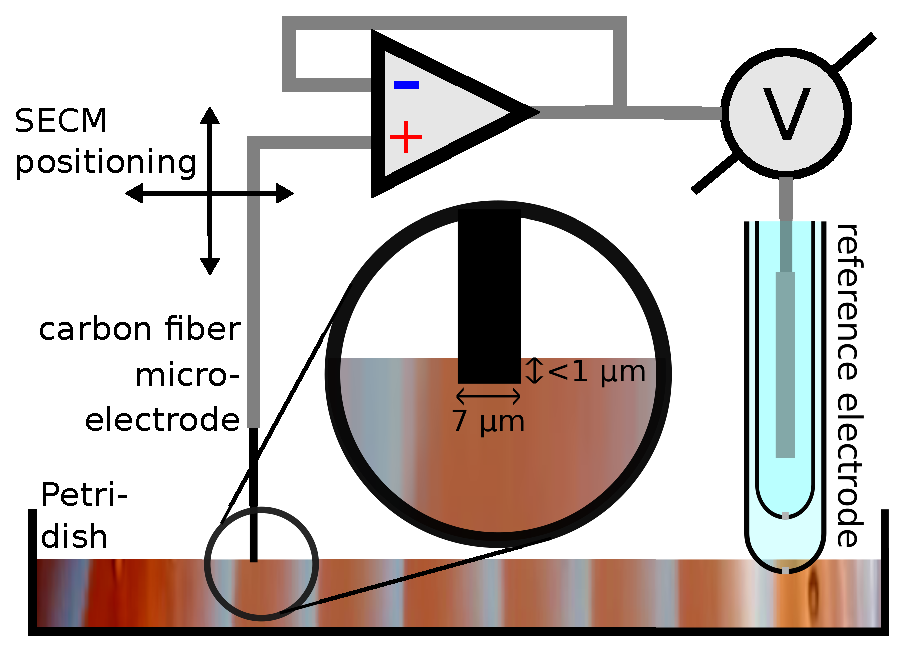
\includegraphics[width=0.45\textwidth]{setup.eps}

\begin{flushleft}
\textbf{B}
\end{flushleft}

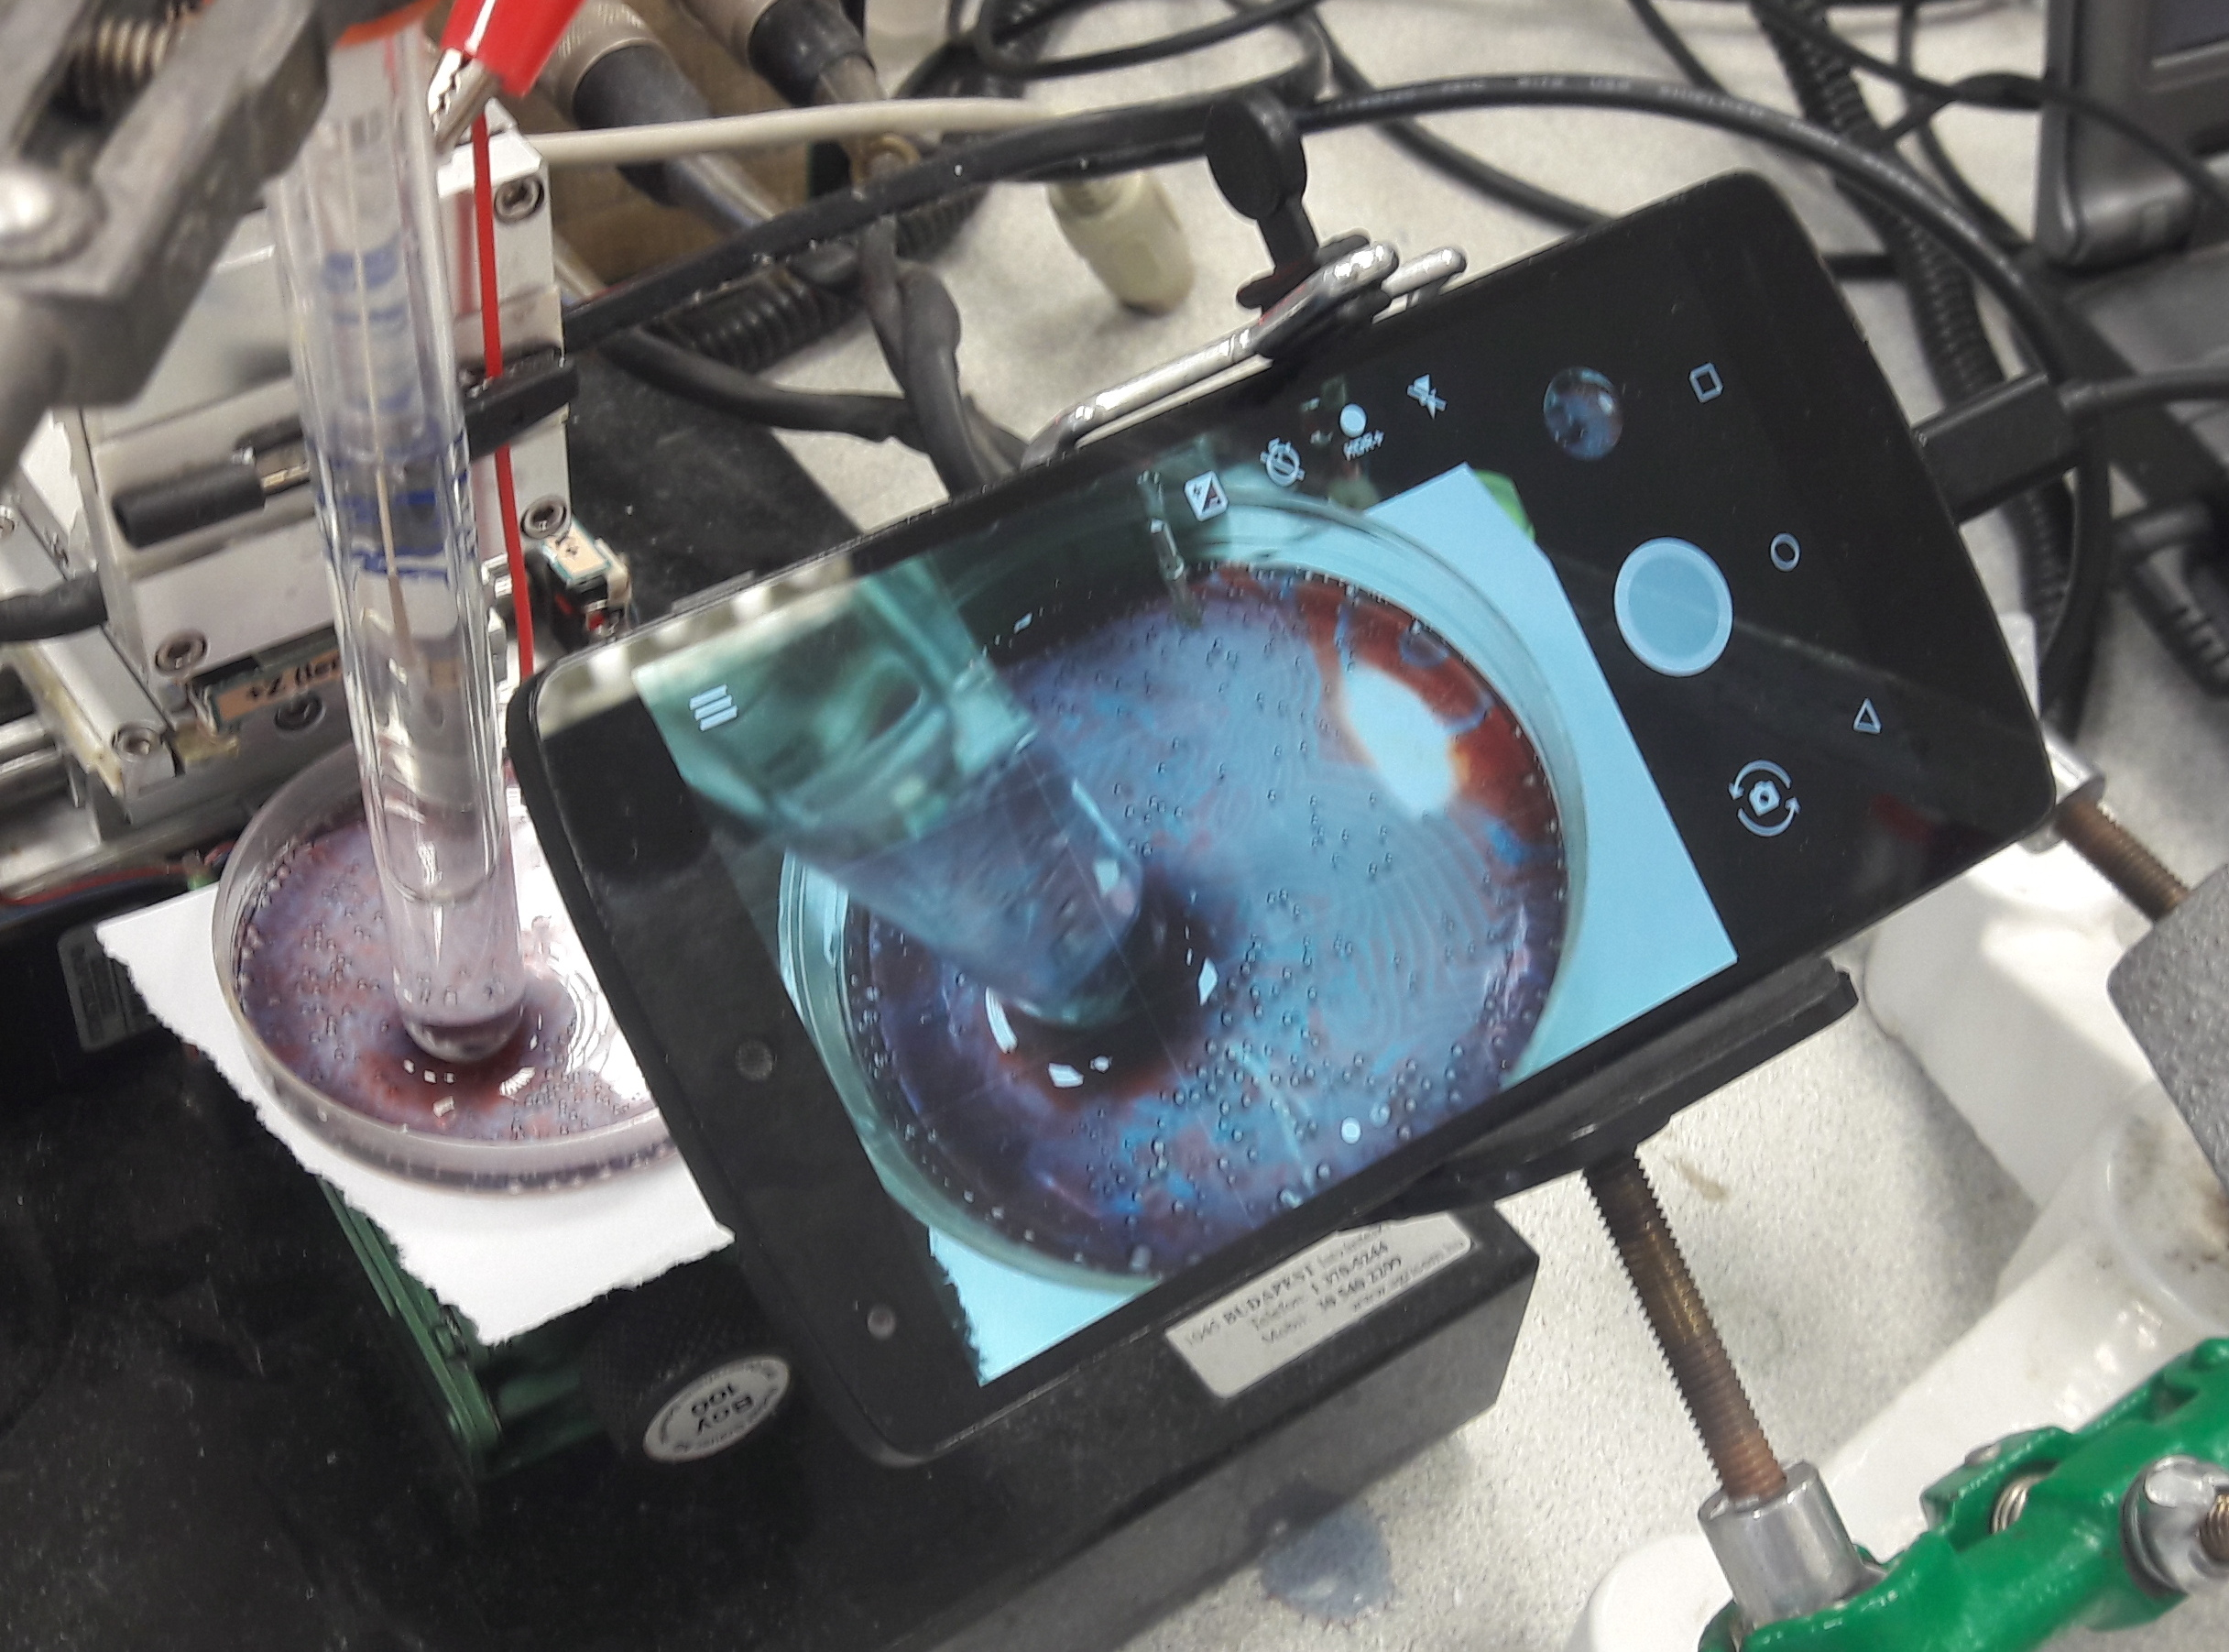
\includegraphics[width=0.45\textwidth]{setup_photo.jpg}
%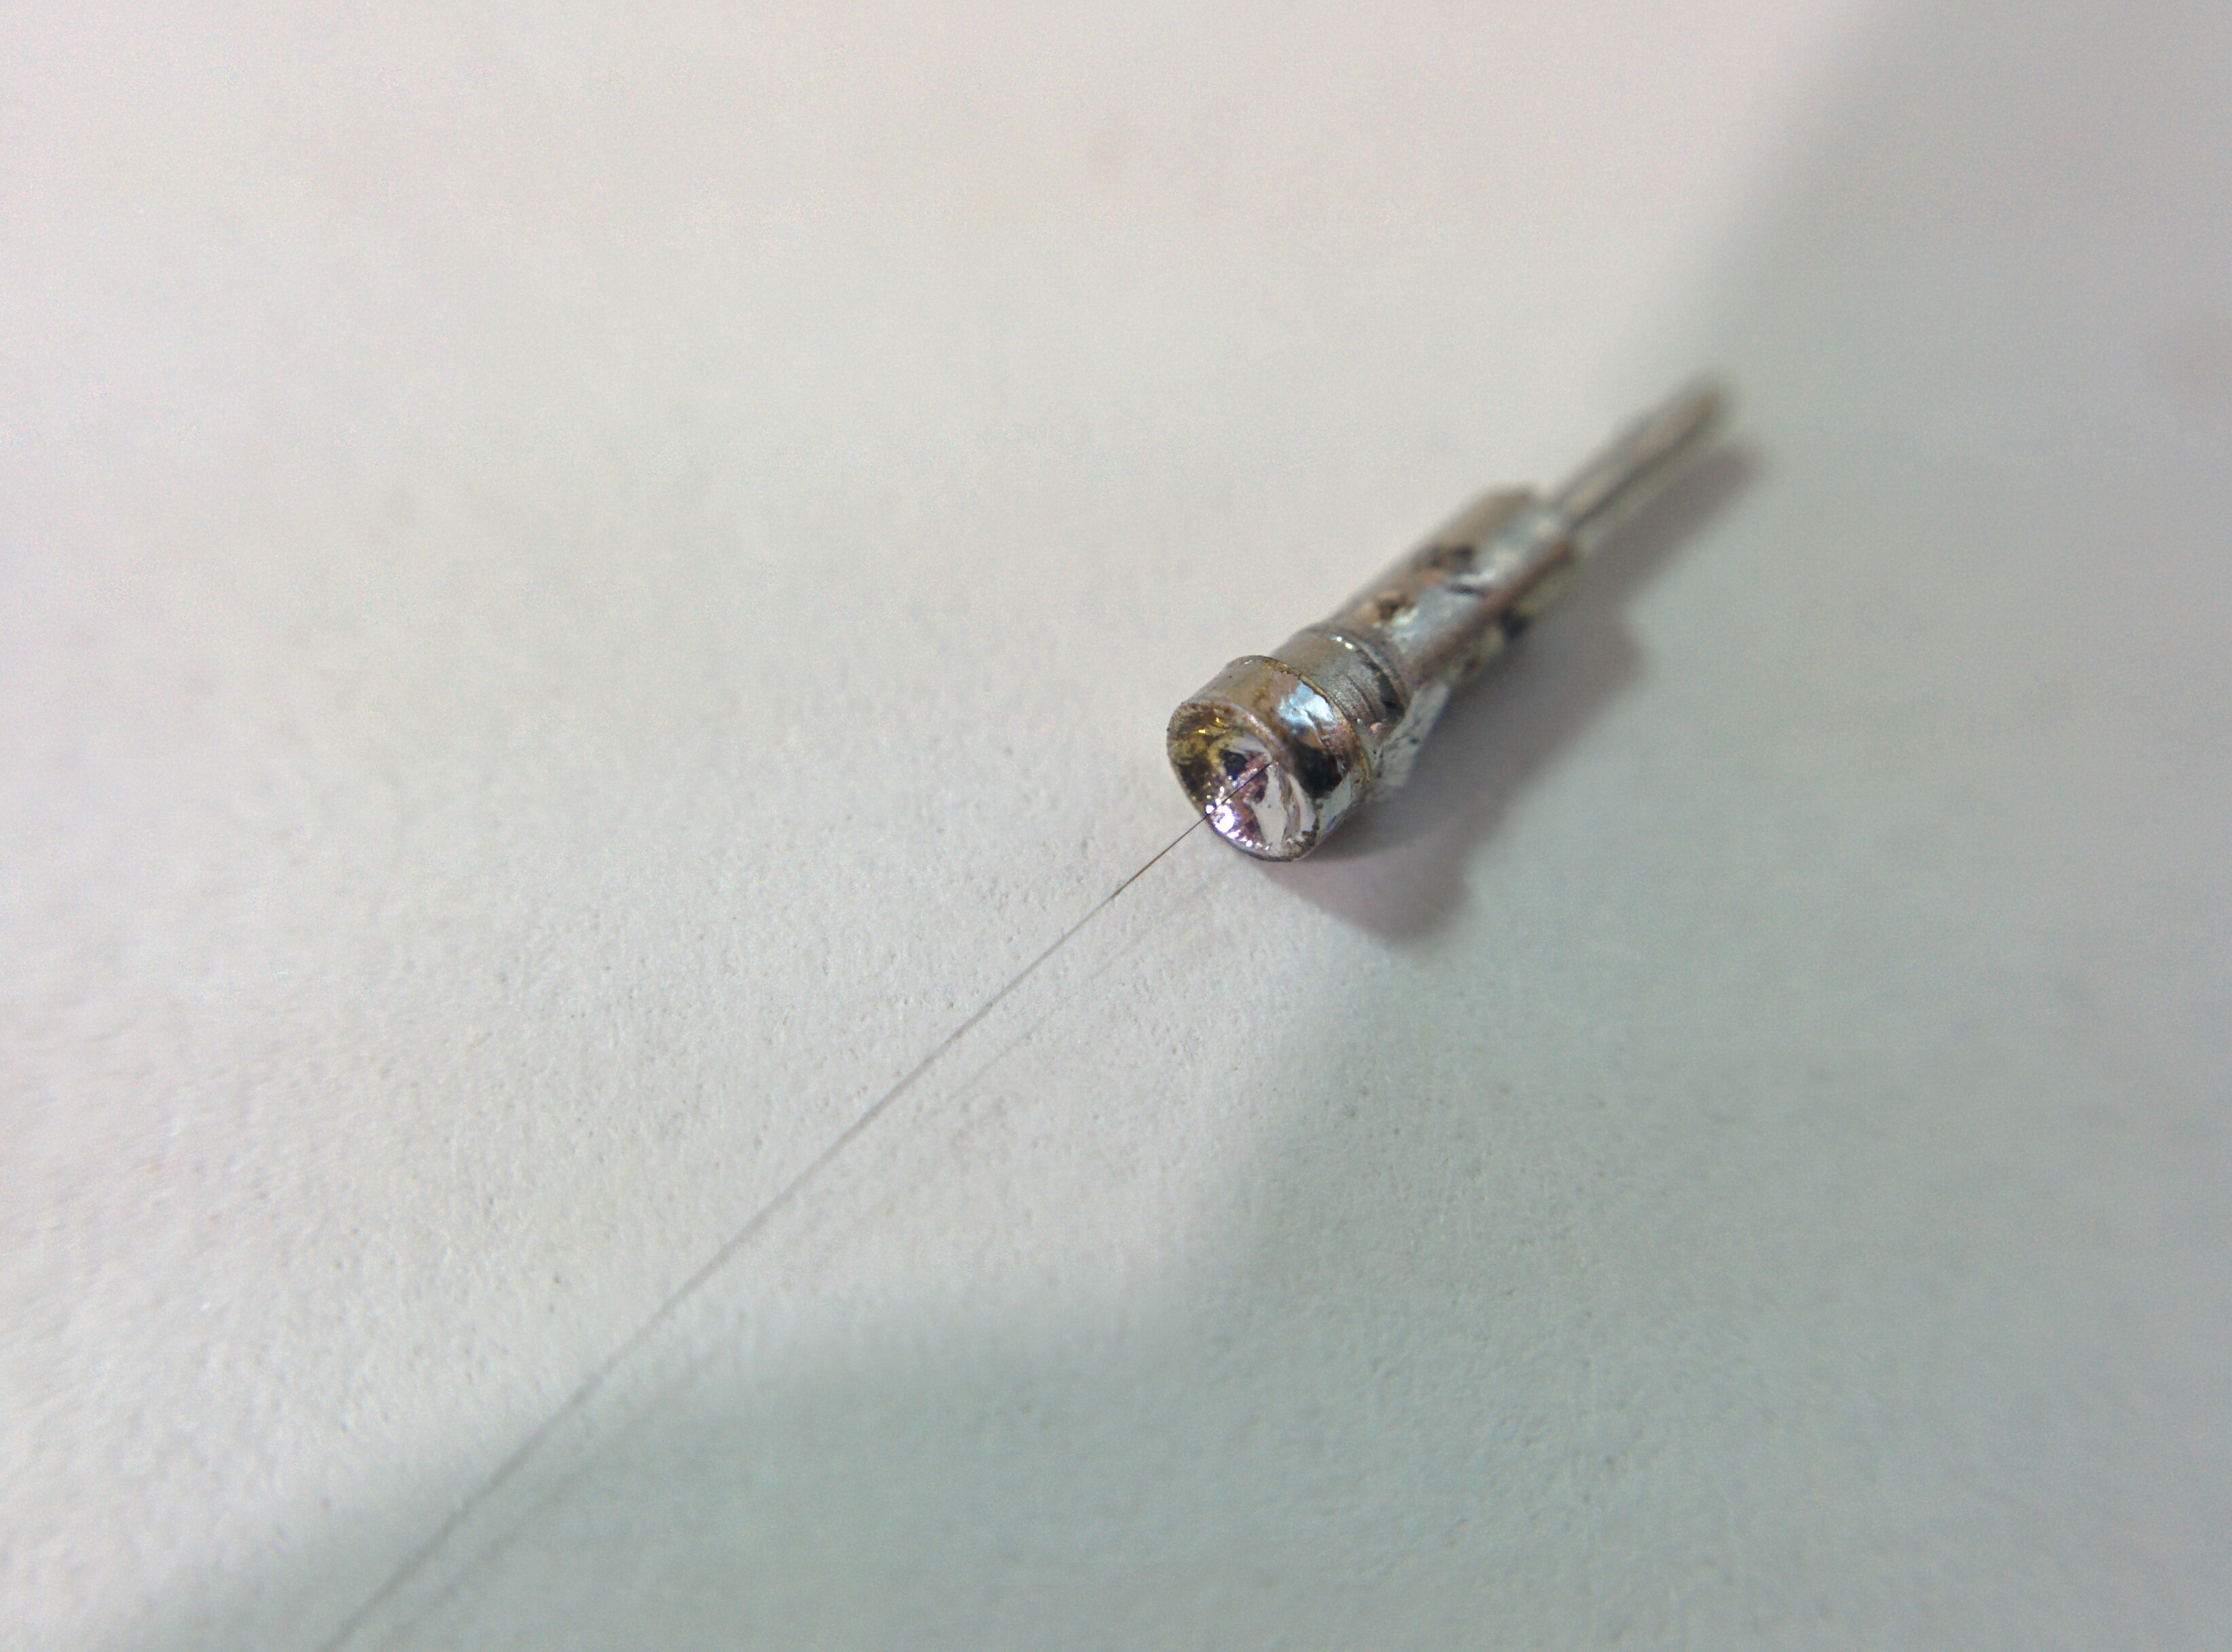
\includegraphics[trim = 200mm 100mm 150mm 200mm, clip, width=0.3\textwidth]{microelectrode.jpg}

\caption{
Sketch (A) and photograph (B) of the experimental setup.
%The carbon fiber microelectrode soldered into the hole of a round female pin header. The diameter of the carbon fiber is 7 $\upmu$m. Since only a less than 1 $\upmu$m portion of the carbon fiber was submersed into the solution, insulation wasn't necessary.
}
\label{fig:setup}
\end{figure}

\paragraph{Optical observation}
The reaction was filmed using an 8 MP Sony Exmor IMX179 1/3.2-inch CMOS sensor (as part of an LG Nexus 5 cell phone), positioned 10 cm from the scanline at a 45 degree angle, with the frame parallel to the scanline.
The space-time plot was prepared using the Blender 2.78 video editing software by grabbing linear, 1 pixel high images from every 30th frame of the video (1 s interval).
The position and orientation of these 1 pixel high frames matched that of the scanline covered by the microelectrode.
The image sequence was assambled by stacking the grabs vertically using Imagemagick 1.3.20.
The overlayed optical-electrochemical plot was created in Gnuplot 4.6.6.

%\begin{table}
% \caption{Initial concentrations of the reactants for the reaction.}
% \label{table:recipe}
% \centering
% \begin{tabular}{r c}
%  Reactant & Concentration \\
%  \hline
%  1 & 2 \\
% \end{tabular}
%\end{table}


\section{Results and discussion}

Figure \ref{fig:spatiotemporal}A shows the electrochemical spatiotemporal image overlayed on top of the optical one.
A very good correlation can be observed between the changes of the potential of the carbon fiber microelectrode and the propagation of the oxidizing chemical waves that is visible in the optical image.
Figure \ref{fig:grabs2}. shows the encounter of the moving microelectrode with wave \#3.
There is no evidence of any convective disturbance caused by the movement of the microelectrode.
This is important, because the BZ reaction is very sensitive to external influences, and it wouldn't be possible to properly observe it with a technique that would influence the reaction.
It seems like the 7 $\upmu$m microelectrode diameter is small enough that the convective effect is alleviated by diffusion to such an extent, that the reaction behaves as if the microelectrode wasn't there.

%Photographs of the reaction mixture at time instances marked by (a)--(b) (in Fig. \ref{fig:spatiotemporal}A) can be seen in Fig. \ref{fig:grabs}.
%These are the starting points of the first four scan cycles.
%At point (a), the microelectrode is at the starting point (marked by the green dot) of the first scan cycle, before any (lateral) tip movement has occured.
%Points (b)--(c) are representing a state where one ,two, and three consecutive scan cycles has benn completed.
%Even after these, the shape of the oxidizing waves is unchanged.
%Fig. \ref{fig:spatiotemporal}B depicts the potential changes of the microelectrode between (a) and (b).

Parameters that can be determined from the optical data -- such as the travel speed of chemical waves -- can also be calculated from the SECM spatiotemporal measurements.
In case of stationary microelectrode, two of them would be necessary at a known distance from each other to calculate the travel speed.
It could be calculated as the ratio of the distance between the electrodes, and the time it takes for the wave to get from the first microelectrode to the second.
However, using the SECM, one microelectrode is sufficient because the tip can be repositioned to allow additional measurements of the same wave.
%The individual waves are numbered in Fig. \ref{fig:spatiotemporal}A.
For instance, wave \#3 was encountered by the carbon microelectrode three times, at t$_1$=47 s, t$_2$=67 s and t$_3$=80 s.
The exact positions of these encounteres are also known: x$_1$=1400 $\upmu$m, x$_2$=6400 $\upmu$m and x$_3$=8600 $\upmu$m.
Based in this data, the average travel speed of wave \#3 during its path between the two outermost positions is 218.18 $\upmu$m/s.
Table \ref{table:stats}. contains several parameters of the waves that were encountered multiple times by the microelectrode. 

\begin{table}
\caption{Chemical wave encounters by the microelectrode during the scanning process.}
\small
\label{table:stats}
\centering
\begin{tabular}{r c c c c c}
% \# & t, s & E, mV & x, mm & \begin{tabular}{c}v, $\upmu$m/s\\ \begin{tabular}{c|c}1--3&1--2, 2--3\end{tabular}\end{tabular}\\
Wave \# & t, s & E, mV & x, mm & v, $\upmu$m/s \\
 \hline
 \hline
% 3&\begin{tabular}{c}47\\67\\80\end{tabular}&\begin{tabular}{c}957\\978\\977\end{tabular}&\begin{tabular}{c}1.4\\6.4\\8.6\end{tabular}&\begin{tabular}{c c}218.8 & \begin{tabular}{c}218.8\\128.8 \end{tabular} \end{tabular}\\
 3&\begin{tabular}{c}47\\67\\80\end{tabular}&\begin{tabular}{c}957\\978\\977\end{tabular}&\begin{tabular}{c}1.4\\6.4\\8.6\end{tabular}&218.8\\
 \hline
 6&\begin{tabular}{c}99\\114\\133.5\end{tabular}&\begin{tabular}{c}968\\975\\1027\end{tabular}&\begin{tabular}{c}1\\4.8\\7.6\end{tabular}&191.3\\
 \hline
 7&\begin{tabular}{c}148.5\\171\\181.5\end{tabular}&\begin{tabular}{c}1052\\1127\\1059\end{tabular}&\begin{tabular}{c}1.6\\7.2\\8.8\end{tabular}&218.18\\
 \hline
 9&\begin{tabular}{c}200\\219.5\\234.5\end{tabular}&\begin{tabular}{c}1016\\1074\\1016\end{tabular}&\begin{tabular}{c}1.4\\6.2\\8\end{tabular}&191.3\\
 \hline
 12&\begin{tabular}{c}253.5\\268\\287\end{tabular}&\begin{tabular}{c}1060\\1120\\1053\end{tabular}&\begin{tabular}{c}0.4\\5.2\\7.4\end{tabular}&208.96\\
\end{tabular}
\end{table}

Using only one electrode has several advantages over using an array, for instance one doesn't have to worry about the differences between the electrodes.
Furthermore, when using an SECM in such study, the microelectrode can be positioned to any coordinate within the mechanical boundaries of the instrument.

One drawback is that the electrochemical data presented in figure \ref{fig:spatiotemporal}. is rather sparse compared to the optical image beneath.
An obvious improvement would be increasing the scanning speed, to make the scanlines more dense.
This is currently a limitation of the SECM instrument in our laboratory, and is subject to a subsequent paper.

The travel speeds calculated are certainly not accurate, since in the measurement both the temporal ($\delta$t=0.5 s) and the spatial ($\delta$x=200 $\upmu$m) data is discrete, hence the matching values of waves \#3 -- \#7 and waves \#6 -- \#9.

It must be mentioned, that these travel speeds are not radial, but rather measured on a chord of the circular waves.
Knowing that the angle at which the reaction has been filmed is 45 degrees, after determining the angle between the radius and the chord, the actual travel speed can be obtained.
%Since the purpose of these measurements is to show 

\def\s{0.5}
\begin{figure}
%% trim = top left bottom right
\centering
\flushleft{\textbf{\large{A}}}
\includegraphics[trim = 15mm 60mm 0mm 30mm, clip, width=\s\textwidth, angle=-90]{spacetime.eps}
%\vspace{1cm}
\flushleft{\textbf{\large{B}}}
\begin{tikzpicture}
  \begin{axis}[width=7cm, height=5cm, xlabel={x / cm},ylabel={time / s},zlabel={E / V}, zmin=0.9]
    %\addplot3[surf, x filter/.code{\pgfmathparse{\pgfmathresults/10000}}] table {17101308_st_lines.txt};
    \addplot3[very thick, color=red] table {17101308_st_lines_back.txt};
    %\addplot3[thick, color=blue] table {17101308_st_lines_there_zerox.txt};
    %\addplot3[thick, color=red] table {17101308_st_lines_back_zerox.txt};
    %\addplot3[color=blue] table {17101308_st_lines_there_base.txt};
    \addplot3[very thick, color=blue] table {17101308_st_lines_there.txt};
  \end{axis}
\end{tikzpicture}
\caption{(A) Electrochemical space-time plot overlayed on top of the corresponding optical one.
The potential of the carbon fiber microelectrode is shown as a function of spatiotemporal coordinates.
Redox indicator was ferroin.
The optical spatiotemporal image was grayscaled to allow better visibility when overlaying the electrochemical data.
The brighter stripes correspond to the oxidizing waves.
(B) The second scan cycle.
Blue line: forward scan, red line: backwards scan.
%Note the shape of the peaks on the red curve, which is measured in the direction that is opposite to the chemical wave travel.
%The elongated portion of these peaks where the potential is decreasing, is not due to 
}
\label{fig:spatiotemporal}
\end{figure}

%\def\s{0.5}
%\def\left{70}
%\def\bottom{120}
%\def\right{50}
%\def\top{30}
%\begin{figure}
%\centering
%\begin{tikzpicture}
%    \draw (0, 0) node[inner sep=0] {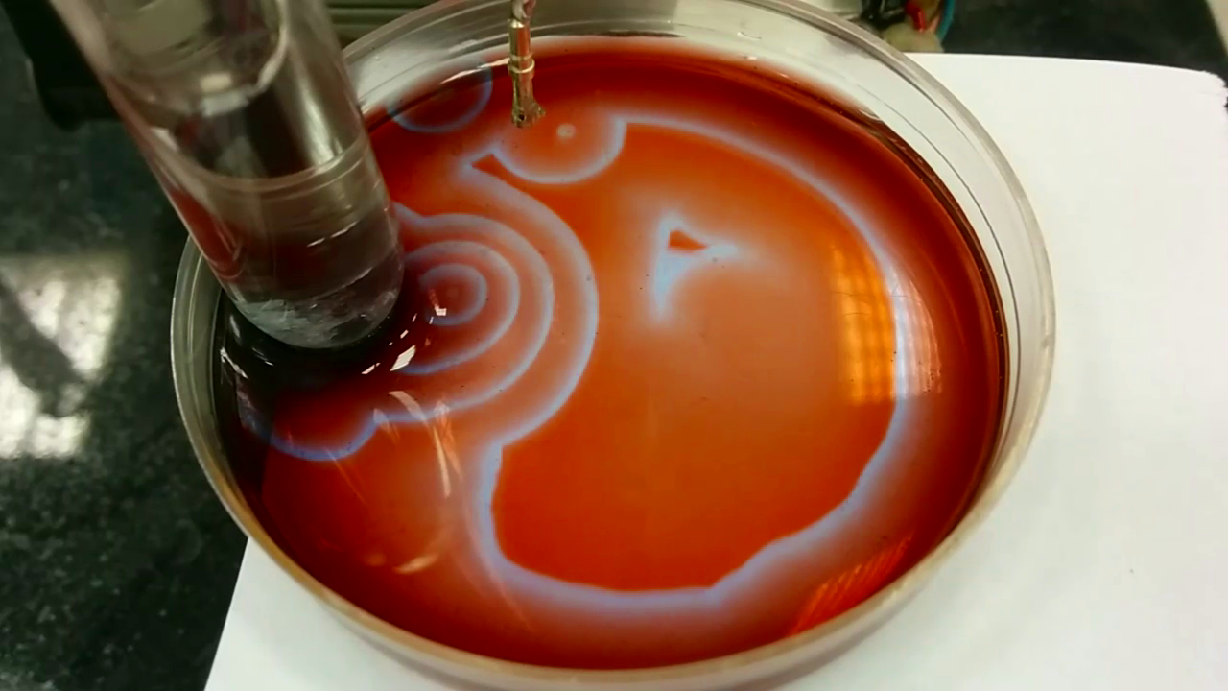
\includegraphics[trim = \left mm \bottom mm \right mm \top mm, clip, width=\s\textwidth]{0.png}};
%    \draw (3.8, 1) node {\textbf{a}};
%    \draw [green] (-1.1,-0.55) node[anchor=south] {\textbf{\large{•}}};
%    \draw [blue] (0.2,-0.55) node[anchor=south] {\textbf{\large{•}}};
%\end{tikzpicture}
%\begin{tikzpicture}
%    \draw (0, 0) node[inner sep=0] {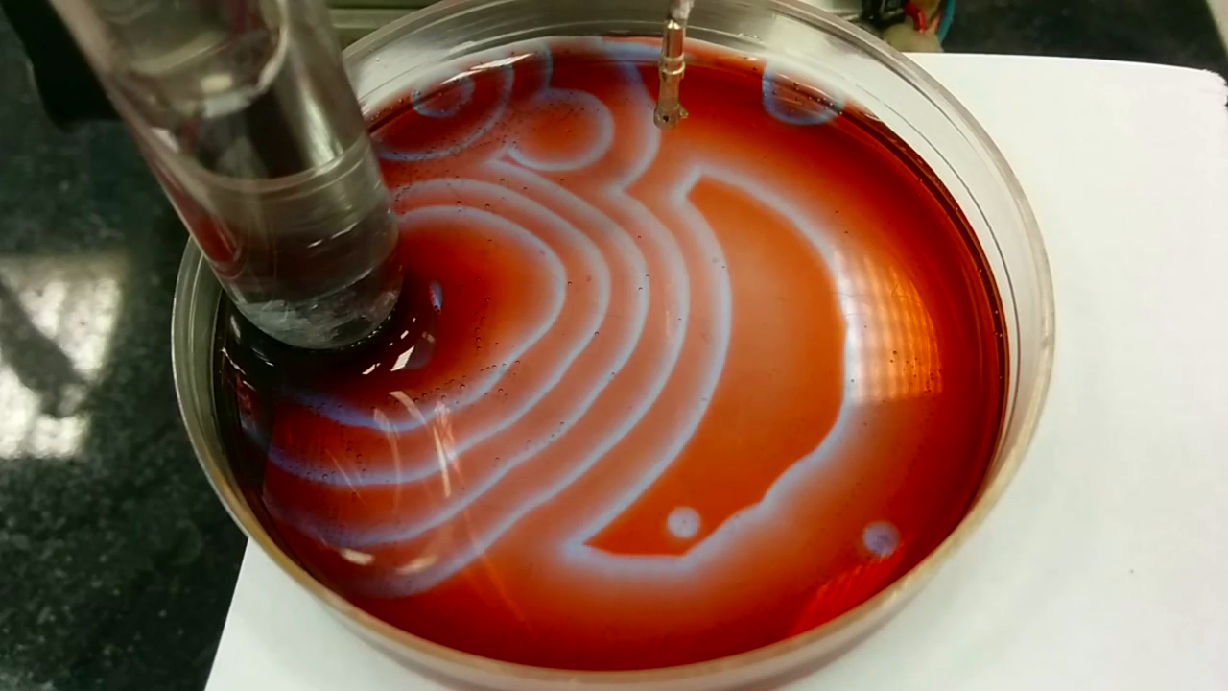
\includegraphics[trim = \left mm \bottom mm \right mm \top mm, clip, width=\s\textwidth]{right.png}};
%    \draw (3.8, 1) node {a};
%    \draw [green] (-1.1,-0.55) node[anchor=south] {\textbf{\large{•}}};
%    \draw [purple] (0.2,-0.55) node[anchor=south] {\textbf{\large{•}}};
%\end{tikzpicture}
%\begin{tikzpicture}
%    \draw (0, 0) node[inner sep=0] {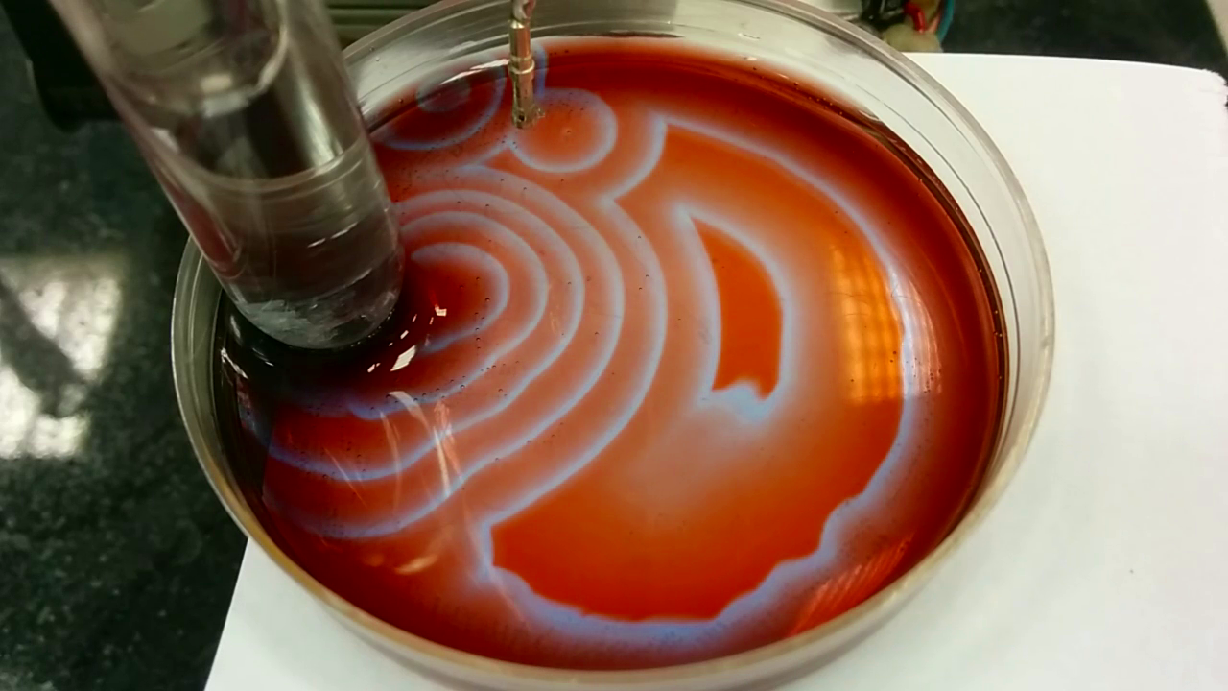
\includegraphics[trim = \left mm \bottom mm \right mm \top mm, clip, width=\s\textwidth]{1.png}};
%    \draw (3.8, 1) node {\textbf{b}};
%    \draw [green] (-1.1,-0.55) node[anchor=south] {\textbf{\large{•}}};
%    \draw [blue] (0.2,-0.55) node[anchor=south] {\textbf{\large{•}}};
%\end{tikzpicture}
%\begin{tikzpicture}
%    \draw (0, 0) node[inner sep=0] {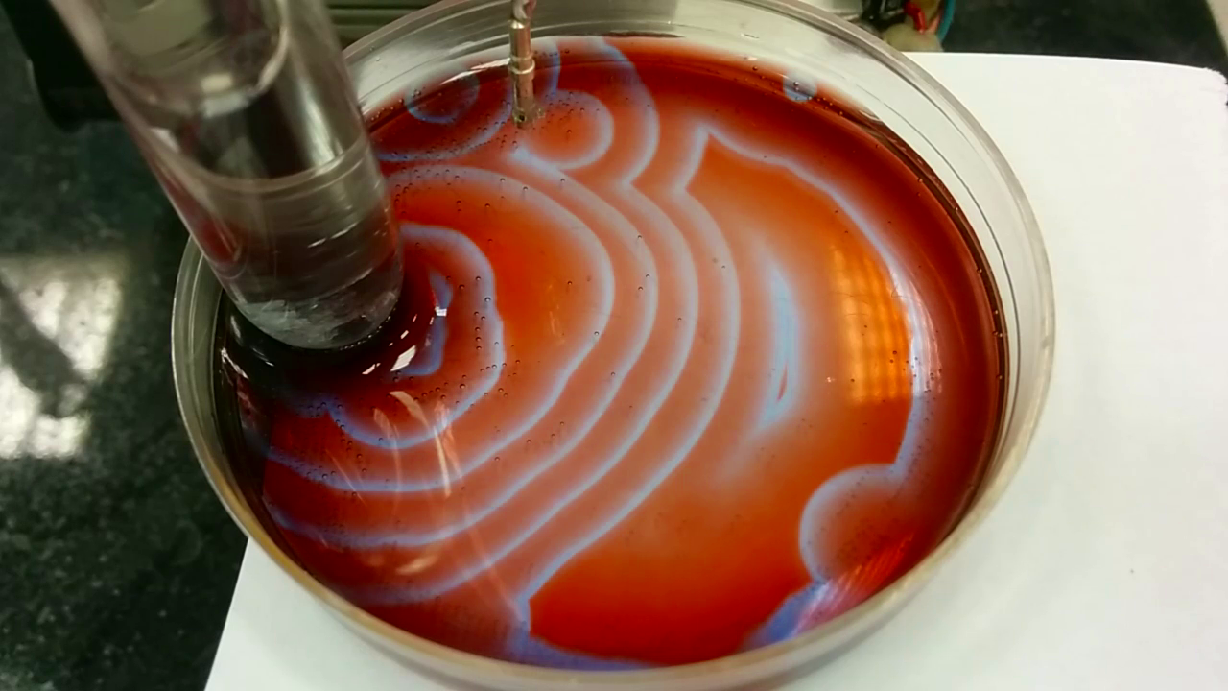
\includegraphics[trim = \left mm \bottom mm \right mm \top mm, clip, width=\s\textwidth]{2.png}};
%    \draw (3.8, 1) node {\textbf{c}};
%    \draw [green] (-1.1,-0.55) node[anchor=south] {\textbf{\large{•}}};
%    \draw [blue] (0.2,-0.55) node[anchor=south] {\textbf{\large{•}}};
%\end{tikzpicture}
%\begin{tikzpicture}
%    \draw (0, 0) node[inner sep=0] {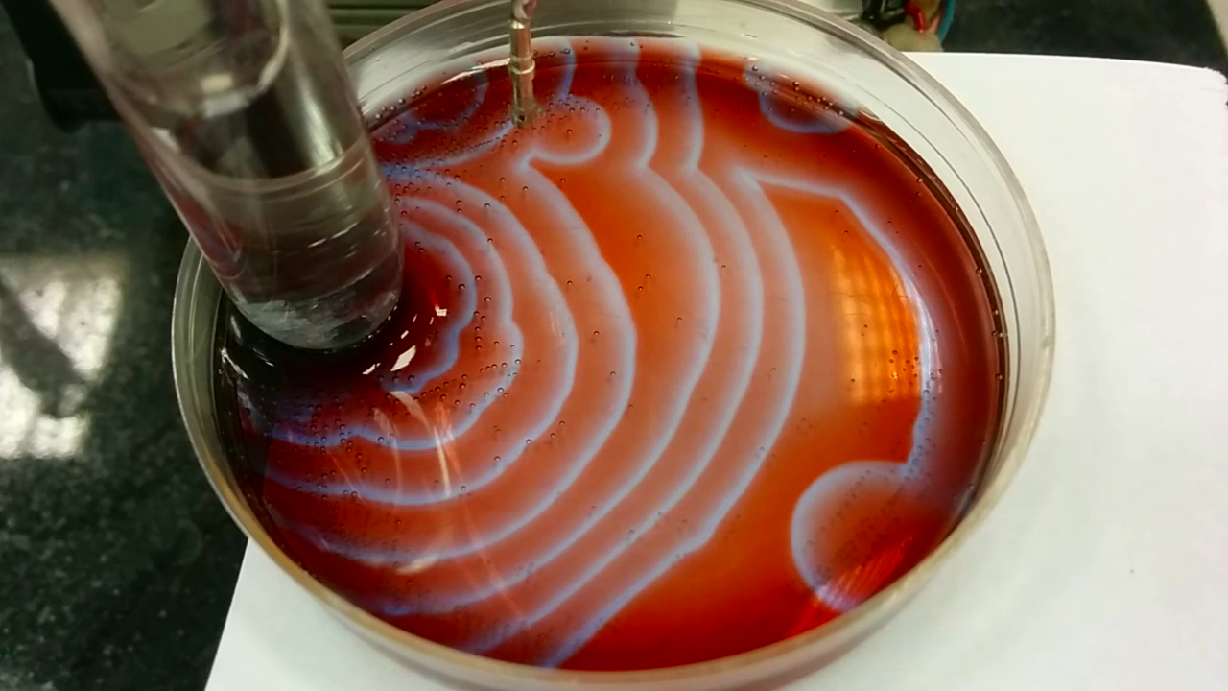
\includegraphics[trim = \left mm \bottom mm \right mm \top mm, clip, width=\s\textwidth]{3.png}};
%    \draw (3.8, 1) node {\textbf{d}};
%    \draw [green] (-1.1,-0.55) node[anchor=south] {\textbf{\large{•}}};
%    \draw [blue] (0.2,-0.55) node[anchor=south] {\textbf{\large{•}}};
%\end{tikzpicture}
%\caption{Frame grabs from the video that was recorded during the experiment.
%(a)--(d): same instances in time as in Fig. \ref{fig:spatiotemporal}.
%(a) t = 0 s (before the first scan cycle), (b) t = 51 s (after the first scan cycle), (c) t = 102 s (after the second scan cycle), (d) t = 153 s (after the third scan cycle).
%Green dot: starting and finishing position of the scan cycle.
%Blue dot: finishing position of the odd numbered scanlines and starting position of the even numbered scanlines.
%In the images, the pin header that was holding the carbon fiber is visible above the green dot.
%Due to its small size, the carbon fiber itself, and the point where it touches the surface of the reaction mixture is invisible in these images.
%On the left side the end of the double wall reference electrode is visible.}
%\label{fig:grabs}
%\end{figure}

%\begin{tikzpicture}
%  \begin{axis}
%    \addplot3[colormap/viridis, surf, very thick] table {17101308_st_lines.txt};
%    %\addplot3[color=black, surf, very thick] table {17101308_st_lines.txt};
%  \end{axis}
%\end{tikzpicture}


%\def\s{0.5}
%\def\left{240}
%\def\bottom{240}
%\def\right{150}
%\def\top{50}
%\begin{figure}
%\centering
%\begin{tikzpicture}
%    \draw (0, 0) node[inner sep=0] {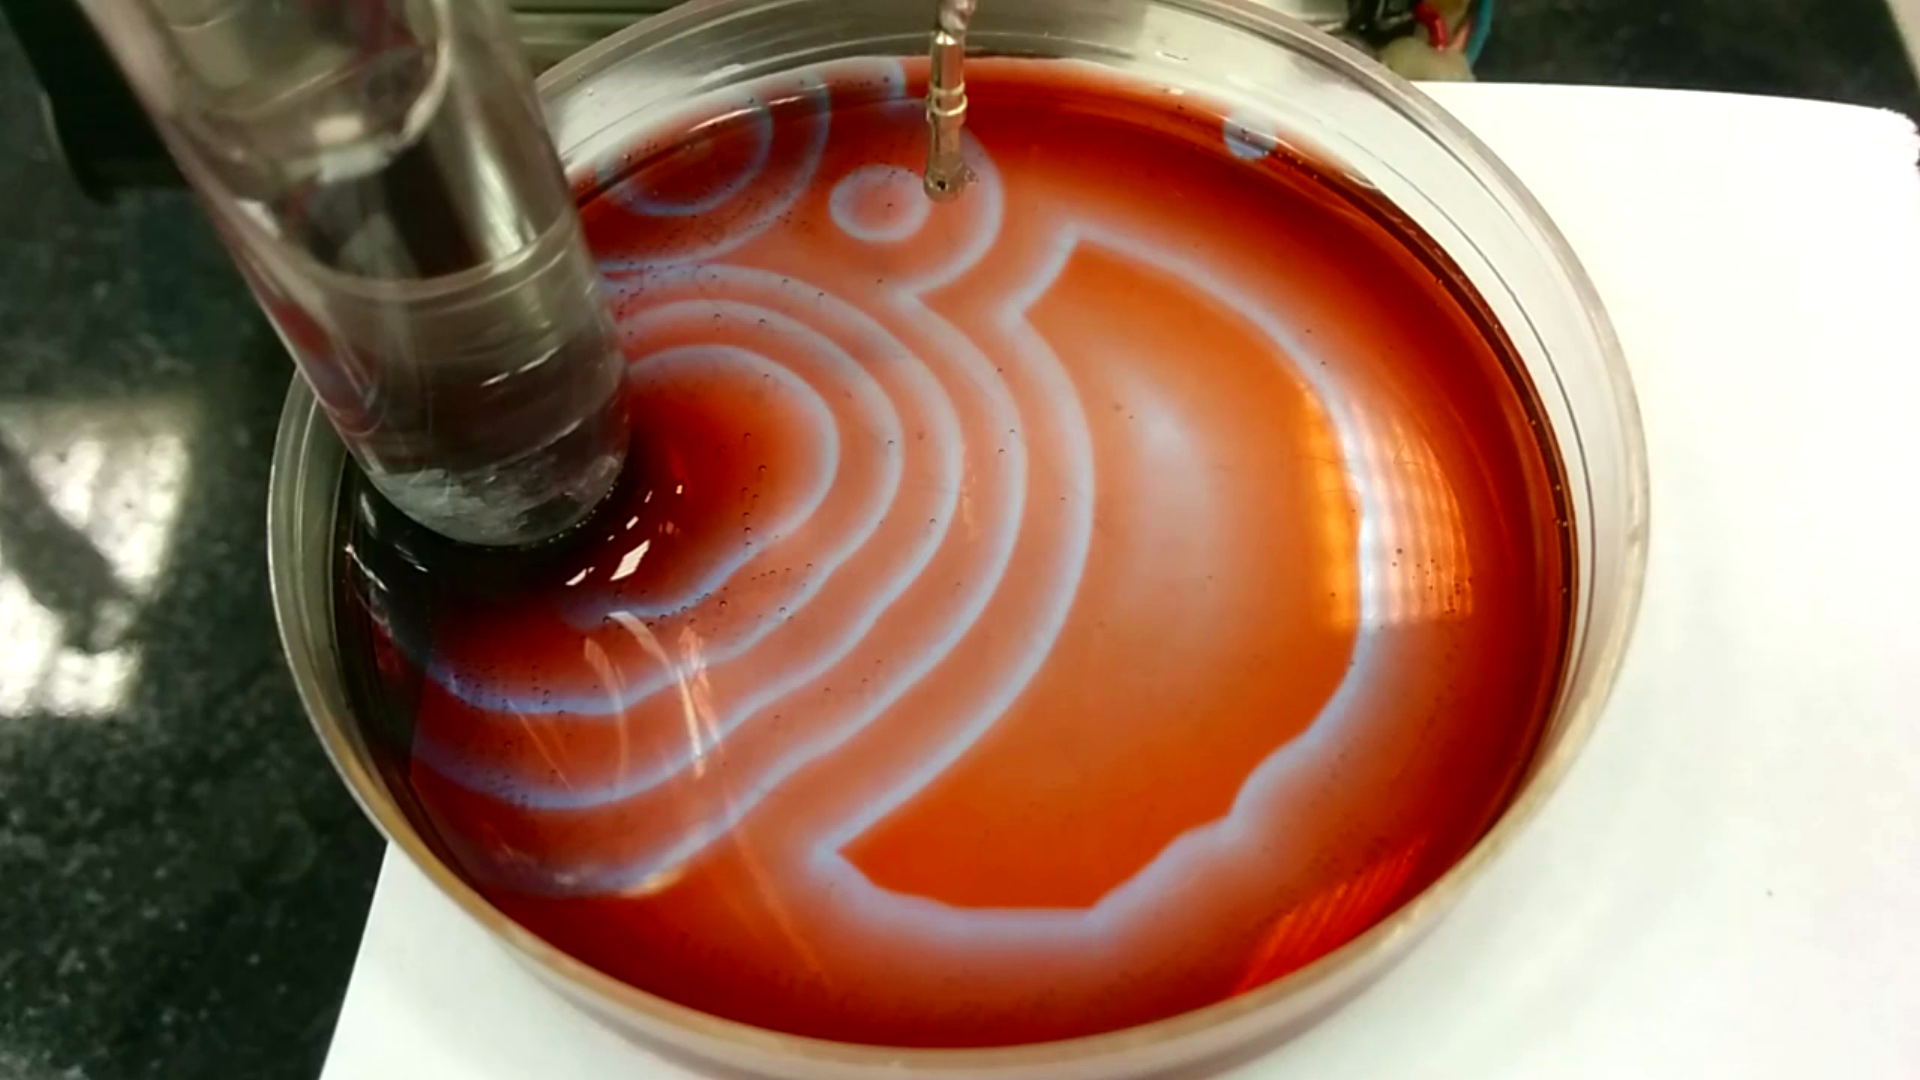
\includegraphics[trim = \left mm \bottom mm \right mm \top mm, clip, width=\s\textwidth]{1988.png}};
    %\draw (3.8, 1) node {\textbf{a}};
    %\draw [green] (-1.1,-0.55) node[anchor=south] {\textbf{\large{•}}};
    %\draw [blue] (0.2,-0.55) node[anchor=south] {\textbf{\large{•}}};
%\end{tikzpicture}
%\begin{tikzpicture}
%    \draw (0, 0) node[inner sep=0] {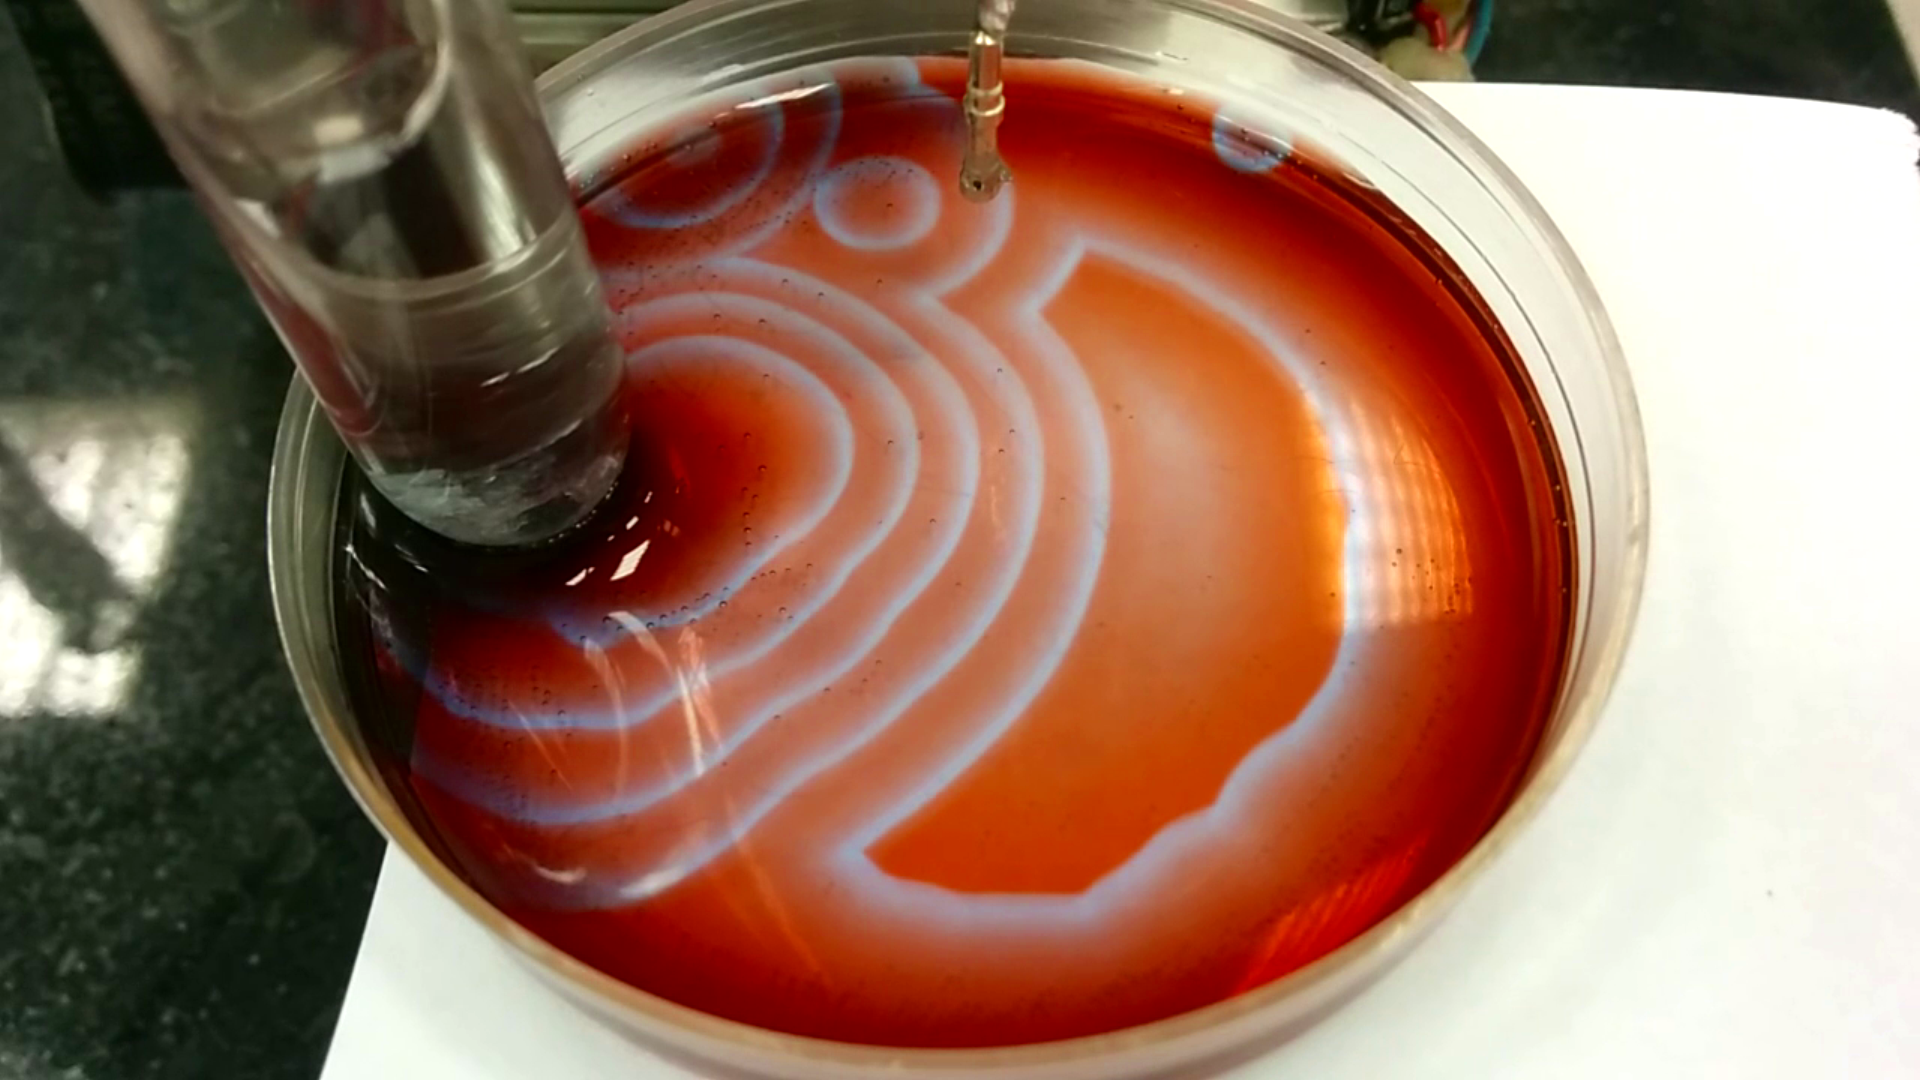
\includegraphics[trim = \left mm \bottom mm \right mm \top mm, clip, width=\s\textwidth]{2108.png}};
    %\draw (3.8, 1) node {\textbf{b}};
    %\draw [green] (-1.1,-0.55) node[anchor=south] {\textbf{\large{•}}};
    %\draw [blue] (0.2,-0.55) node[anchor=south] {\textbf{\large{•}}};
%\end{tikzpicture}
%\begin{tikzpicture}
%    \draw (0, 0) node[inner sep=0] {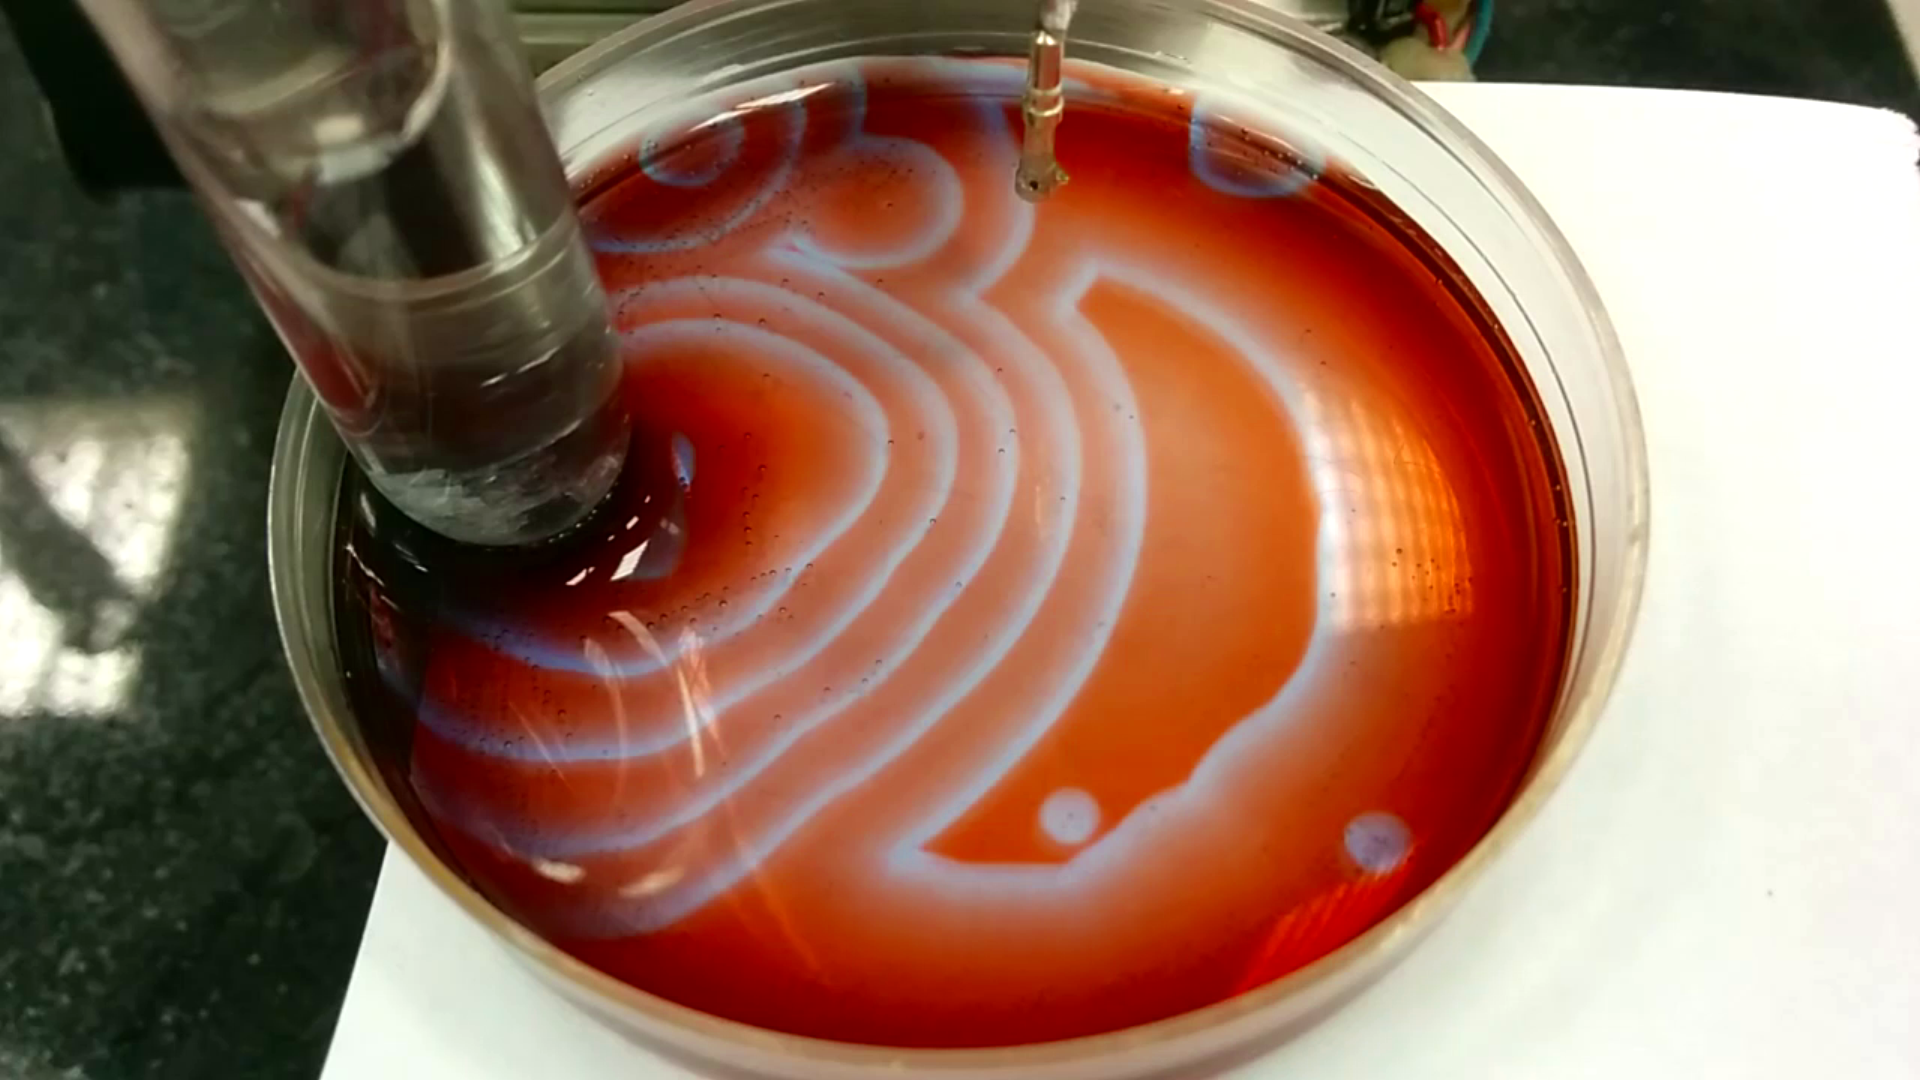
\includegraphics[trim = \left mm \bottom mm \right mm \top mm, clip, width=\s\textwidth]{2357.png}};
    %\draw (3.8, 1) node {\textbf{c}};
    %\draw [green] (-1.1,-0.55) node[anchor=south] {\textbf{\large{•}}};
    %\draw [blue] (0.2,-0.55) node[anchor=south] {\textbf{\large{•}}};
%\end{tikzpicture}
%\begin{tikzpicture}
%    \draw (0, 0) node[inner sep=0] {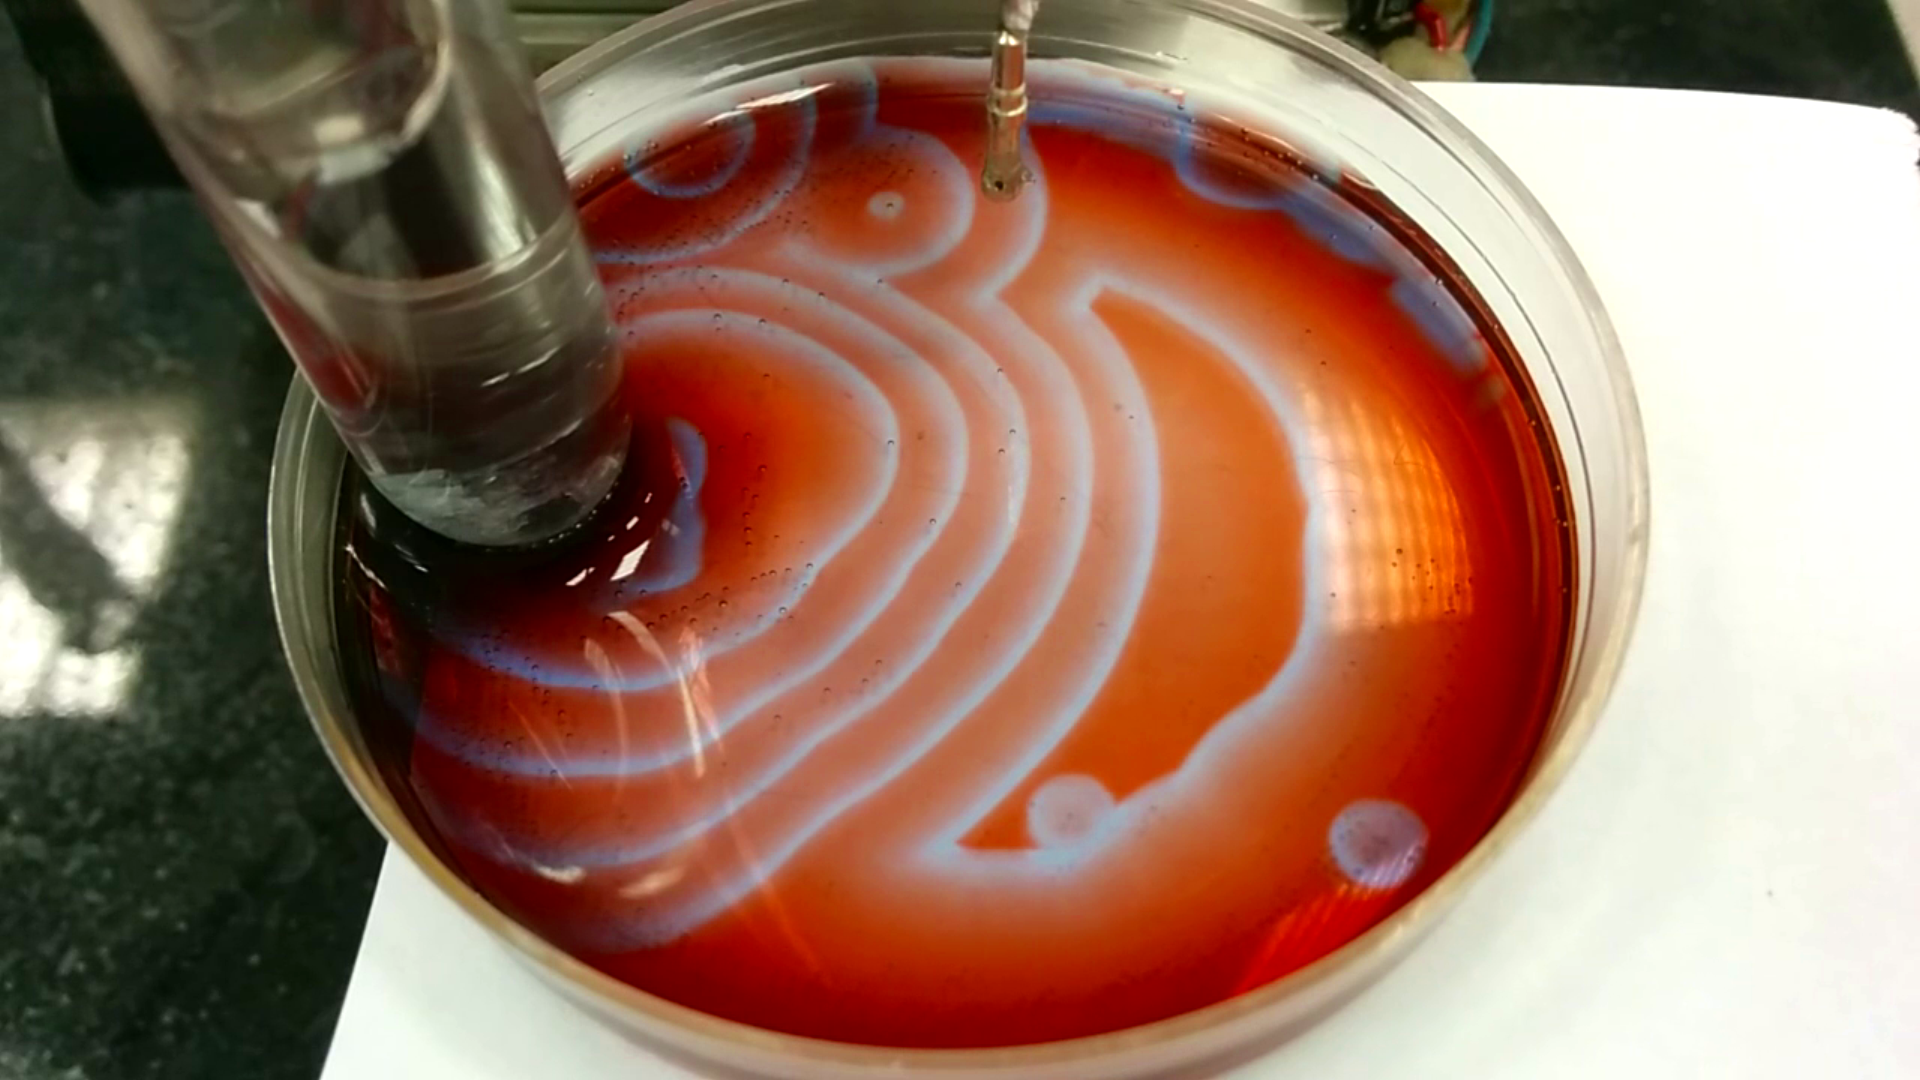
\includegraphics[trim = \left mm \bottom mm \right mm \top mm, clip, width=\s\textwidth]{2477.png}};
    %\draw (3.8, 1) node {\textbf{d}};
    %\draw [green] (-1.1,-0.55) node[anchor=south] {\textbf{\large{•}}};
    %\draw [blue] (0.2,-0.55) node[anchor=south] {\textbf{\large{•}}};
%\end{tikzpicture}
%\begin{tikzpicture}
%    \draw (0, 0) node[inner sep=0] {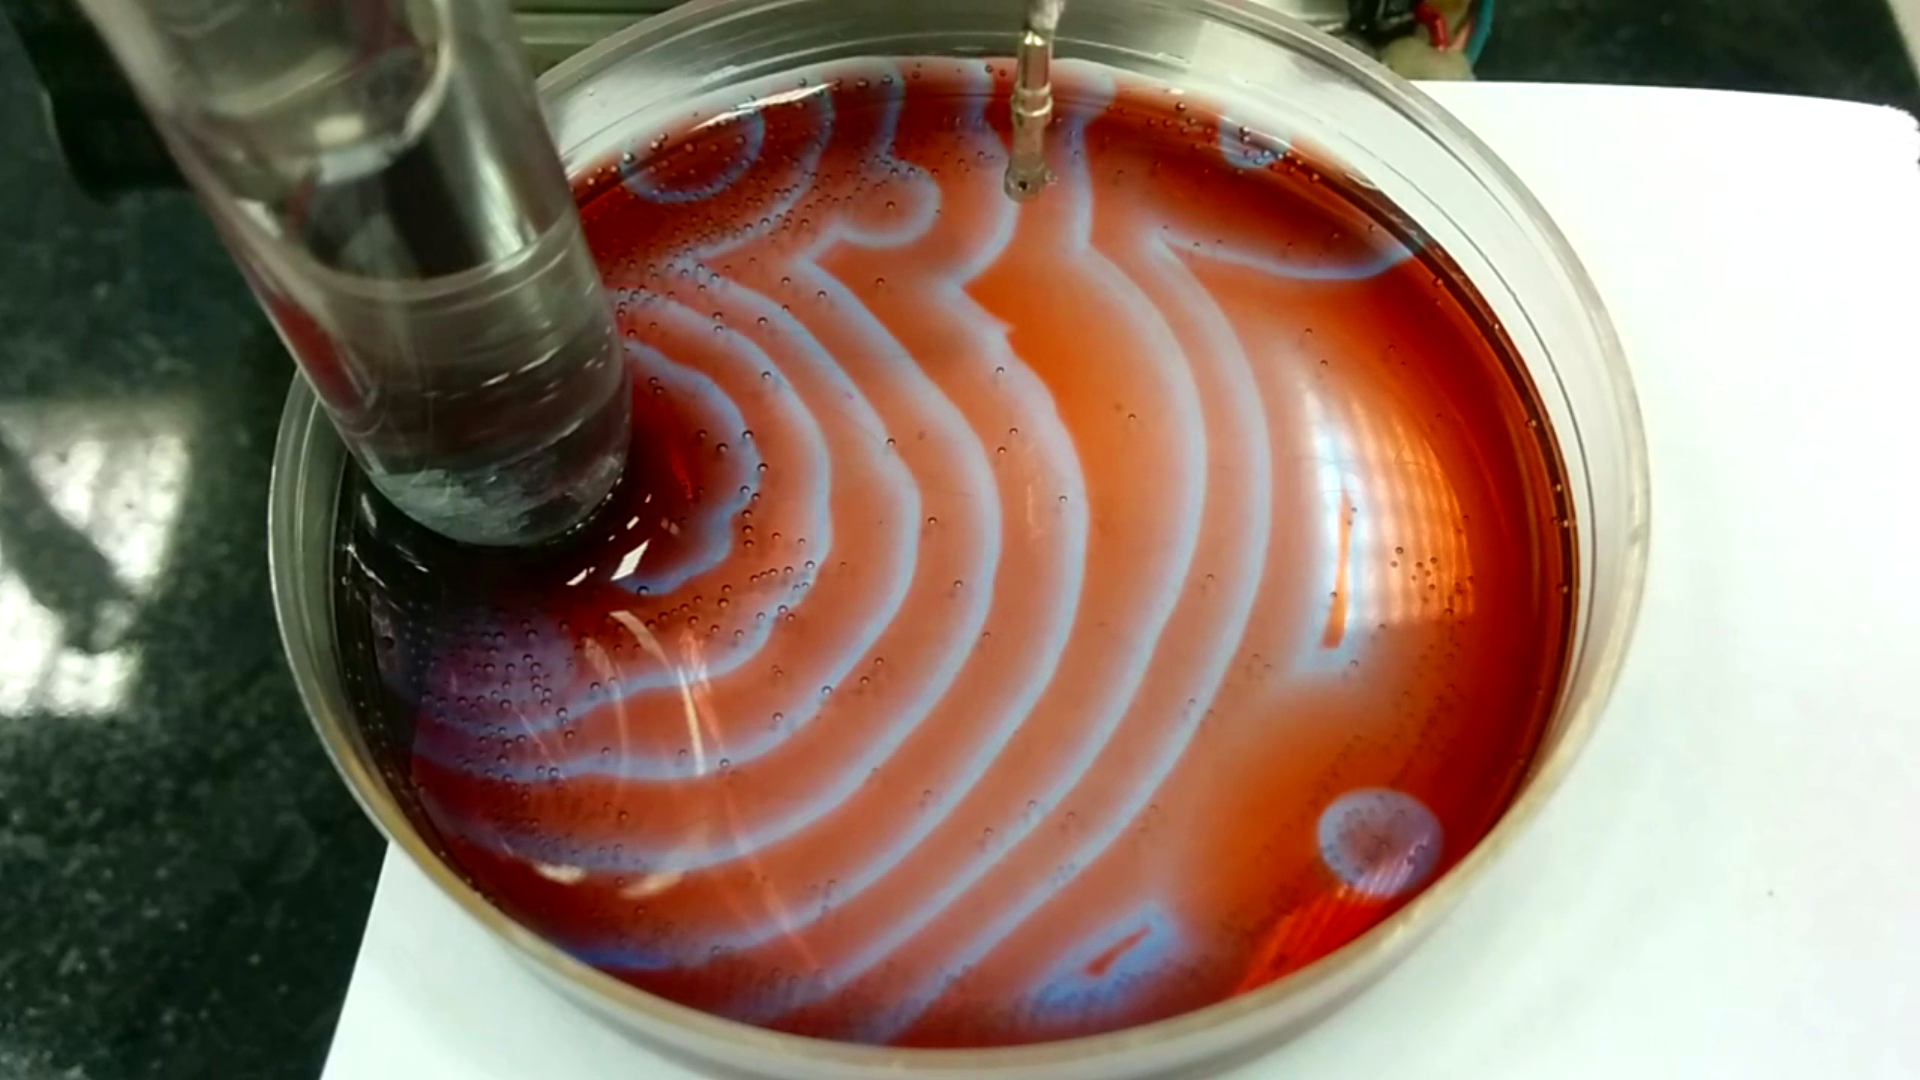
\includegraphics[trim = \left mm \bottom mm \right mm \top mm, clip, width=\s\textwidth]{5351.png}};
    %\draw (3.8, 1) node {\textbf{d}};
    %\draw [green] (-1.1,-0.55) node[anchor=south] {\textbf{\large{•}}};
    %\draw [blue] (0.2,-0.55) node[anchor=south] {\textbf{\large{•}}};
%\end{tikzpicture}
%\caption{Frame grabs from the video that was recorded during the experiment.
%(a)--(d): same instances in time as in Fig. \ref{fig:spatiotemporal}.
%(a) t = 0 s (before the first scan cycle), (b) t = 51 s (after the first scan cycle), (c) t = 102 s (after the second scan cycle), (d) t = 153 s (after the third scan cycle).
%Green dot: starting and finishing position of the scan cycle.
%Blue dot: finishing position of the odd numbered scanlines and starting position of the even numbered scanlines.
%In the images, the pin header that was holding the carbon fiber is visible above the green dot.
%Due to its small size, the carbon fiber itself, and the point where it touches the surface of the reaction mixture is invisible in these images.
%On the left side the end of the double wall reference electrode is visible.}
%\label{fig:grabs}
%\end{figure}

\begin{figure}
\centering
\begin{tikzpicture}
    %\draw (0, 0) node[inner sep=0] {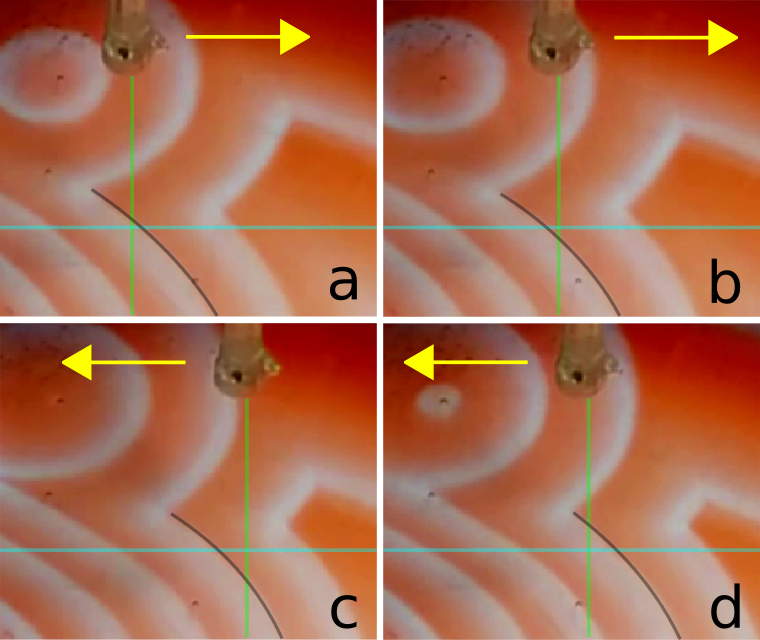
\includegraphics[trim={2cm 0cm 2cm 0 }, clip,width=\s\textwidth]{grabs.png}};
    \draw (0, 0) node[inner sep=0] {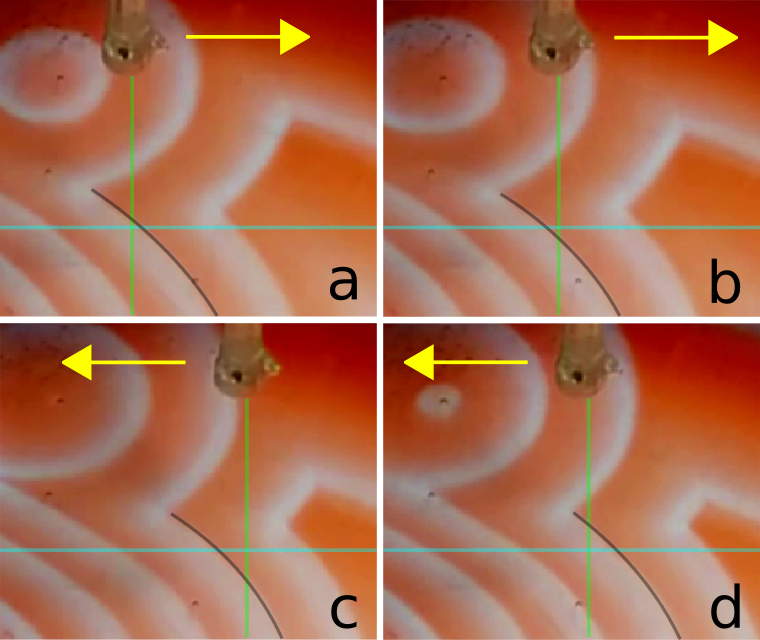
\includegraphics[width=0.45\textwidth]{grabs.png}};
    %\draw (3.8, 1) node {\textbf{a}};
    %\draw [green] (-1.1,-0.55) node[anchor=south] {\textbf{\large{•}}};
    %\draw [blue] (0.2,-0.55) node[anchor=south] {\textbf{\large{•}}};
\end{tikzpicture}
\caption{Frame grabs from the video that was recorded during the experiment.
%(a)--(d): same instances in time as in Fig. \ref{fig:spatiotemporal}.
%(a) t = 0 s (before the first scan cycle), (b) t = 51 s (after the first scan cycle), (c) t = 102 s (after the second scan cycle), (d) t = 153 s (after the third scan cycle).
%Green dot: starting and finishing position of the scan cycle.
%Blue dot: finishing position of the odd numbered scanlines and starting position of the even numbered scanlines.
Numbers represent the order of the chemical waves, same as in figure \ref{fig:spatiotemporal}.
(a)--(b) 2 seconds before and after the carbon fiber reaches wave \#3 while traveling in the same direction.
(c)--(d) 2 seconds before and after the carbon fiber reaches wave \#3 while traveling in the opposite direction.
Due to its small size, the carbon fiber itself, and the point where it touches the surface of the reaction mixture is invisible in these images.
The green -- vertical -- line reperesents the \emph{y}-coordinate of the point where the carbon fiber touches the surface.
The blue -- horizontal -- line marks the scanline.
Wave \#3 is marked by the black line.
The pin header that was holding the carbon fiber is visible in the top portion of the images.
%On the left side the end of the double junction reference electrode is visible.
}
\label{fig:grabs2}
\end{figure}

\section{Conclusions}
Potentiometry has been used to study the BZ reaction almost since its discovery.
Compared to the optical methods, it allowed farther reaching conclusions to be made by several research groups.
There is however one area where electrochemical investigations certainly lacked; they couldn't provide spatial information, which 2D photometry or tomography could easily do.
In this paper, we made an attempt to combine the advantages of the two techniques.
In its current form there are several limitations of the technique, for instance, the relatively low density of the electrochemical data.
Further development can be expected.

By using potentiometric SECM with a sufficiently small microelectrode, the redox potential can be spatially resolved in a quasy-2D BZ reaction, without influencing the reaction.
By substituting the indicator tip or combining multiple ones, other parameters can be measured, possibly simultaneously.
With an appropriately small ion-selective microelectrode, bromide-ion activity could be mapped in the BZ reaction.
There are several extensive works on the use of such ion-selective electrodes in the study of the BZ and other oscillating reactions \cite{noszticzius1, noszticzius2}.
A pH-sensitive antimony microelectrode with a less than 7 $\upmu$m diameter can be easily prepared.
It could be used as an indicator microprobe to map pH in pH-regulated oscillators \cite{orban}.
This could provide an opportunity to further advance our understanding of the BZ and other oscillating reactions.

\section*{Acknowledgements}
The work was financially supported by the National Research, Development and Innovation Office (Budapest, Hungary) under grant K125244.
András Kiss is thankful for the inspiring discussions with Gyula Hoffmann about pattern formation.
\section*{References}

\begin{thebibliography}{5}
\bibitem{bansagi2011}Bánsági, Tamás, Vladimir K. Vanag, and Irving R. Epstein. "Tomography of reaction-diffusion microemulsions reveals three-dimensional Turing patterns." Science 331.6022 (2011): 1309-1312.

\bibitem{belousov}Belousov, B. P. "Sbornik Referatov po Radiatsionni Meditsine." Medgiz, Moscow 145 (1958).

\bibitem{zaikin1970}Zaikin, A. N., and A. M. Zhabotinsky. "Concentration wave propagation in two-dimensional liquid-phase self-oscillating system." Nature 225.5232 (1970): 535-537.

\bibitem{fkn1}Noyes, Richard M., Richard Field, and Endre Kőrös. "Oscillations in chemical systems. I. Detailed mechanism in a system showing temporal oscillations." Journal of the American Chemical Society 94.4 (1972): 1394-1395.

\bibitem{fkn2}Field, Richard J., Endre Kőrös, and Richard M. Noyes. "Oscillations in chemical systems. II. Thorough analysis of temporal oscillation in the bromate-cerium-malonic acid system." Journal of the American Chemical Society 94.25 (1972): 8649-8664.

%\bibitem{hess1} Nagy-Ungvarai, Zs, et al. "Experimental study of spiral waves in the cerium-catalyzed Belousov-Zhabotinskii reaction." Journal of physical chemistry 94.24 (1990): 8677-8682.

\bibitem{hess2}Nagy-Ungvárai, Zs, H. Baumgärtl, and B. Hess. "Electrochemical detection of pattern formation in the Belousov-Zhabotinskii reaction." Chemical Physics Letters 168.6 (1990): 539-542. 

\bibitem{hess3}Nagy-Ungvárai, Zsuzsanna, and Benno Hess. "Control of dynamic pattern formation in the Belousov-Zhabotinsky reaction." Physica D: Nonlinear Phenomena 49.1-2 (1991): 33-39.

\bibitem{winfree}Winfree, Arthur T. The geometry of biological time. Vol. 12. Springer Science \& Business Media, 2001.

\bibitem{phd}András, Kiss. "Recent Advances in Potenciometric Scanning Electrochemical Microscopy." PhD Dissertation, University of Pécs, (2017).

\bibitem{noszticzius1}Noszticzius, Z., E. Noszticzius, and Z. A. Schelly. "Use of ion-selective electrodes for monitoring oscillating reactions. 1. Potential response of the silver halide membrane electrodes to hypohalous acids." Journal of the American Chemical Society 104.23 (1982): 6194-6199.

\bibitem{noszticzius2}Noszticzius, Z., E. Noszticzius, and Z. A. Schelly. "Use of ion-selective electrodes for monitoring oscillating reactions. 2. Potential response of bromide-iodide-selective electrodes in slow corrosive processes. Disproportionation of bromous and iodous acids. A Lotka-Volterra model for the halate driven oscillators." The Journal of Physical Chemistry 87.3 (1983): 510-524.

\bibitem{orban}Orbán, Miklós, Krisztina Kurin-Csörgei, and Irving R. Epstein. "pH-regulated chemical oscillators." Accounts of chemical research 48.3 (2015): 593-601.
\end{thebibliography}
\end{document}
